\documentclass[11pt,tikz,border=5pt]{standalone}

\usepackage[european,siunitx,EFvoltages]{circuitikz}

\begin{document}
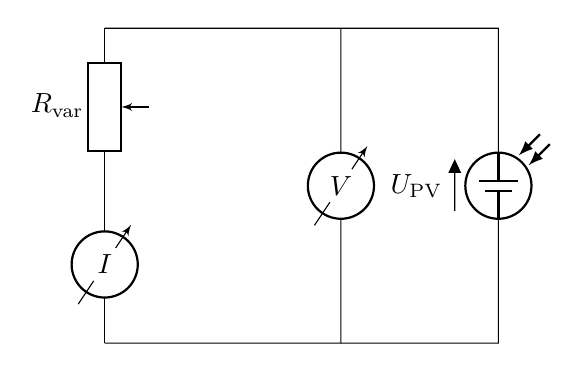
\begin{tikzpicture}[yscale=2]
  \draw (2, 0) to[potentiometer, name=P, l_=$R_\text{var}$] ++(0, -1) to[rmeterwa, t=$I$] ++(0, -1);
  \draw (2, 0) -- ++(3, 0) to[rmeterwa, t=$V$] ++(0, -2) -- (2, -2);)
  \draw (5, -2) -- ++(2, 0) to[pvsource,v=$U_\text{PV}$] ++(0, 2) -- ++(-2, 0);
\end{tikzpicture}
\end{document}